\documentclass[a4paper, 11pt, twoside=semi]{scrartcl}

\usepackage[utf8]{inputenc}
\usepackage[english]{babel}

\usepackage{enumerate}

% Deutsche Silbentrennung
%\usepackage[ngerman]{babel}

% Typische Mathesymbole etc, was man oft braucht
\usepackage{textcomp}
\usepackage{latexsym}
\usepackage{amssymb}
\usepackage{amsmath}
\usepackage{wasysym}
%\usepackage{txfonts}

% Teilfiguren in figure Umgebungen erlauben%
\usepackage{subfig}
\usepackage{float}
\restylefloat{figure}

% Schrift die mit Zeichencodierung klar kommt
%\usepackage{lmodern}




% Bilder einfügen
\usepackage{graphicx}
% Quelltext einfügen
\usepackage{verbatim}
%allows multiple rows and colums in a tabular environment
\usepackage{array}
%\usepackage{multirow}
\usepackage{multicol}


% Definitionen von Farben
\usepackage{xcolor}

% Einf\"ugen von Tikz grafiken
\usepackage{booktabs}
\usepackage{pgf}
\usepackage{tikz}
\usetikzlibrary{shapes,backgrounds,mindmap,trees,calc}

\usepackage{pgfplots}
%\usepackage{pgfplotstable}
%\usepgfplotslibrary{colormaps}
%\usepgfplotslibrary{colorbrewer}
\usetikzlibrary{pgfplots.colorbrewer}
\pgfplotsset{compat=1.15} %
\pgfplotsset{cycle list/PiYG}
\pgfplotsset{cycle list/Spectral}
\pgfplotsset{cycle list/Greys}

\author{Thomas Kühn}
\title{Evaluation Methods and Replicability of Software
Architecture Research Objects}
\subtitle{Generated Figures Shown in the Paper}

\begin{document}

\maketitle

\section{Number of research objects from 2017 to 2021}

%\subsection{Portfolio f\"ur Year und Research Object (Gr\"o\ss{}e entspricht der Anzahl)}
%\begin{figure}
\begin{center}
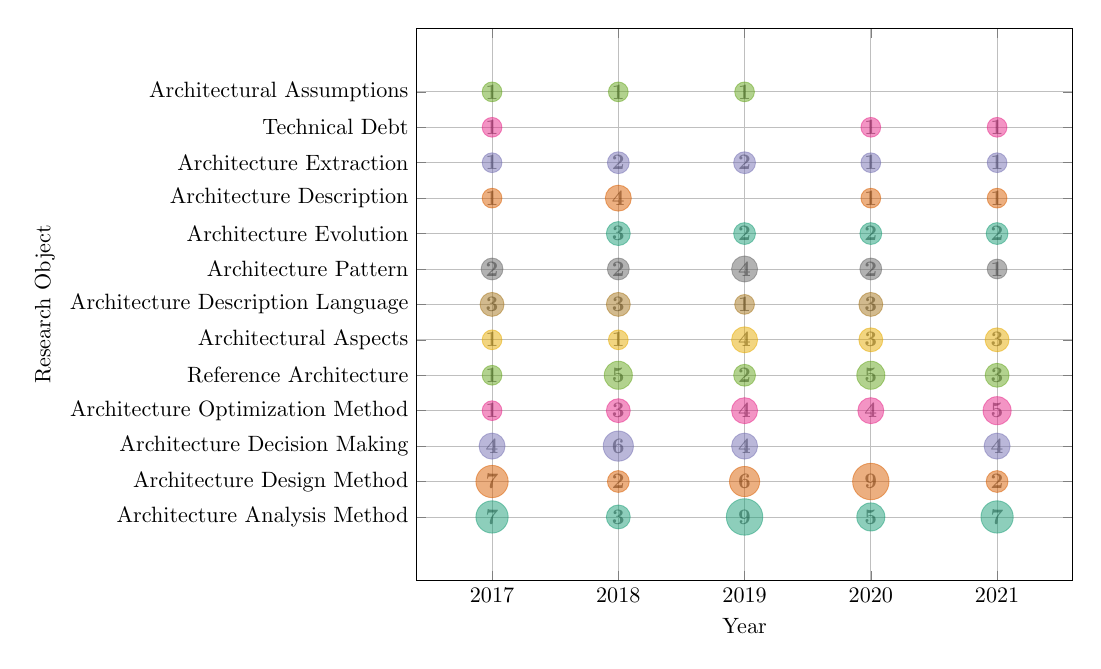
\begin{tikzpicture}[scale=.8]
\pgfplotsset{cycle list/Dark2}
\begin{axis}[width=.99\linewidth,
    enlargelimits=0.15,
    %x tick label style={rotate=45,anchor=east},
    xtick={0,1,2,3,4}, xticklabels={2017,2018,2019,2020,2021},
    xlabel={Year},
    ytick={0,1,2,3,4,5,6,7,8,9,10,11,12}, yticklabels={Architecture Analysis Method,Architecture Design Method,Architecture Decision Making,Architecture Optimization Method,Reference Architecture,Architectural Aspects,Architecture Description Language,Architecture Pattern,Architecture Evolution,Architecture Description,Architecture Extraction,Technical Debt,Architectural Assumptions},
    ylabel={Research Object},
    grid=both,
    scatter,scatter src=y,
    scatter/classes={0={draw=Dark2-A,fill=Dark2-A}, 1={draw=Dark2-B,fill=Dark2-B}, 2={draw=Dark2-C,fill=Dark2-C}, 3={draw=Dark2-D,fill=Dark2-D}, 4={draw=Dark2-E,fill=Dark2-E}, 5={draw=Dark2-F,fill=Dark2-F}, 6={draw=Dark2-G,fill=Dark2-G}, 7={draw=Dark2-H,fill=Dark2-H}, 8={draw=Dark2-A,fill=Dark2-A}, 9={draw=Dark2-B,fill=Dark2-B}, 10={draw=Dark2-C,fill=Dark2-C}, 11={draw=Dark2-D,fill=Dark2-D}, 12={draw=Dark2-E,fill=Dark2-E}}
]

\addplot+[mark=*,mark size=7.294,opacity=0.5,text=black] coordinates { (0,0) } node[text=black,font=\bfseries] {7};
\addplot+[mark=*,mark size=7.294,opacity=0.5,text=black] coordinates { (0,1) } node[text=black,font=\bfseries] {7};
\addplot+[mark=*,mark size=5.882,opacity=0.5,text=black] coordinates { (0,2) } node[text=black,font=\bfseries] {4};
\addplot+[mark=*,mark size=4.471,opacity=0.5,text=black] coordinates { (0,3) } node[text=black,font=\bfseries] {1};
\addplot+[mark=*,mark size=4.471,opacity=0.5,text=black] coordinates { (0,4) } node[text=black,font=\bfseries] {1};
\addplot+[mark=*,mark size=4.471,opacity=0.5,text=black] coordinates { (0,5) } node[text=black,font=\bfseries] {1};
\addplot+[mark=*,mark size=5.412,opacity=0.5,text=black] coordinates { (0,6) } node[text=black,font=\bfseries] {3};
\addplot+[mark=*,mark size=4.941,opacity=0.5,text=black] coordinates { (0,7) } node[text=black,font=\bfseries] {2};
\addplot+[mark=*,mark size=4.471,opacity=0.5,text=black] coordinates { (0,9) } node[text=black,font=\bfseries] {1};
\addplot+[mark=*,mark size=4.471,opacity=0.5,text=black] coordinates { (0,10) } node[text=black,font=\bfseries] {1};
\addplot+[mark=*,mark size=4.471,opacity=0.5,text=black] coordinates { (0,11) } node[text=black,font=\bfseries] {1};
\addplot+[mark=*,mark size=4.471,opacity=0.5,text=black] coordinates { (0,12) } node[text=black,font=\bfseries] {1};
\addplot+[mark=*,mark size=5.412,opacity=0.5,text=black] coordinates { (1,0) } node[text=black,font=\bfseries] {3};
\addplot+[mark=*,mark size=4.941,opacity=0.5,text=black] coordinates { (1,1) } node[text=black,font=\bfseries] {2};
\addplot+[mark=*,mark size=6.824,opacity=0.5,text=black] coordinates { (1,2) } node[text=black,font=\bfseries] {6};
\addplot+[mark=*,mark size=5.412,opacity=0.5,text=black] coordinates { (1,3) } node[text=black,font=\bfseries] {3};
\addplot+[mark=*,mark size=6.353,opacity=0.5,text=black] coordinates { (1,4) } node[text=black,font=\bfseries] {5};
\addplot+[mark=*,mark size=4.471,opacity=0.5,text=black] coordinates { (1,5) } node[text=black,font=\bfseries] {1};
\addplot+[mark=*,mark size=5.412,opacity=0.5,text=black] coordinates { (1,6) } node[text=black,font=\bfseries] {3};
\addplot+[mark=*,mark size=4.941,opacity=0.5,text=black] coordinates { (1,7) } node[text=black,font=\bfseries] {2};
\addplot+[mark=*,mark size=5.412,opacity=0.5,text=black] coordinates { (1,8) } node[text=black,font=\bfseries] {3};
\addplot+[mark=*,mark size=5.882,opacity=0.5,text=black] coordinates { (1,9) } node[text=black,font=\bfseries] {4};
\addplot+[mark=*,mark size=4.941,opacity=0.5,text=black] coordinates { (1,10) } node[text=black,font=\bfseries] {2};
\addplot+[mark=*,mark size=4.471,opacity=0.5,text=black] coordinates { (1,12) } node[text=black,font=\bfseries] {1};
\addplot+[mark=*,mark size=8.235,opacity=0.5,text=black] coordinates { (2,0) } node[text=black,font=\bfseries] {9};
\addplot+[mark=*,mark size=6.824,opacity=0.5,text=black] coordinates { (2,1) } node[text=black,font=\bfseries] {6};
\addplot+[mark=*,mark size=5.882,opacity=0.5,text=black] coordinates { (2,2) } node[text=black,font=\bfseries] {4};
\addplot+[mark=*,mark size=5.882,opacity=0.5,text=black] coordinates { (2,3) } node[text=black,font=\bfseries] {4};
\addplot+[mark=*,mark size=4.941,opacity=0.5,text=black] coordinates { (2,4) } node[text=black,font=\bfseries] {2};
\addplot+[mark=*,mark size=5.882,opacity=0.5,text=black] coordinates { (2,5) } node[text=black,font=\bfseries] {4};
\addplot+[mark=*,mark size=4.471,opacity=0.5,text=black] coordinates { (2,6) } node[text=black,font=\bfseries] {1};
\addplot+[mark=*,mark size=5.882,opacity=0.5,text=black] coordinates { (2,7) } node[text=black,font=\bfseries] {4};
\addplot+[mark=*,mark size=4.941,opacity=0.5,text=black] coordinates { (2,8) } node[text=black,font=\bfseries] {2};
\addplot+[mark=*,mark size=4.941,opacity=0.5,text=black] coordinates { (2,10) } node[text=black,font=\bfseries] {2};
\addplot+[mark=*,mark size=4.471,opacity=0.5,text=black] coordinates { (2,12) } node[text=black,font=\bfseries] {1};
\addplot+[mark=*,mark size=6.353,opacity=0.5,text=black] coordinates { (3,0) } node[text=black,font=\bfseries] {5};
\addplot+[mark=*,mark size=8.235,opacity=0.5,text=black] coordinates { (3,1) } node[text=black,font=\bfseries] {9};
\addplot+[mark=*,mark size=5.882,opacity=0.5,text=black] coordinates { (3,3) } node[text=black,font=\bfseries] {4};
\addplot+[mark=*,mark size=6.353,opacity=0.5,text=black] coordinates { (3,4) } node[text=black,font=\bfseries] {5};
\addplot+[mark=*,mark size=5.412,opacity=0.5,text=black] coordinates { (3,5) } node[text=black,font=\bfseries] {3};
\addplot+[mark=*,mark size=5.412,opacity=0.5,text=black] coordinates { (3,6) } node[text=black,font=\bfseries] {3};
\addplot+[mark=*,mark size=4.941,opacity=0.5,text=black] coordinates { (3,7) } node[text=black,font=\bfseries] {2};
\addplot+[mark=*,mark size=4.941,opacity=0.5,text=black] coordinates { (3,8) } node[text=black,font=\bfseries] {2};
\addplot+[mark=*,mark size=4.471,opacity=0.5,text=black] coordinates { (3,9) } node[text=black,font=\bfseries] {1};
\addplot+[mark=*,mark size=4.471,opacity=0.5,text=black] coordinates { (3,10) } node[text=black,font=\bfseries] {1};
\addplot+[mark=*,mark size=4.471,opacity=0.5,text=black] coordinates { (3,11) } node[text=black,font=\bfseries] {1};
\addplot+[mark=*,mark size=7.294,opacity=0.5,text=black] coordinates { (4,0) } node[text=black,font=\bfseries] {7};
\addplot+[mark=*,mark size=4.941,opacity=0.5,text=black] coordinates { (4,1) } node[text=black,font=\bfseries] {2};
\addplot+[mark=*,mark size=5.882,opacity=0.5,text=black] coordinates { (4,2) } node[text=black,font=\bfseries] {4};
\addplot+[mark=*,mark size=6.353,opacity=0.5,text=black] coordinates { (4,3) } node[text=black,font=\bfseries] {5};
\addplot+[mark=*,mark size=5.412,opacity=0.5,text=black] coordinates { (4,4) } node[text=black,font=\bfseries] {3};
\addplot+[mark=*,mark size=5.412,opacity=0.5,text=black] coordinates { (4,5) } node[text=black,font=\bfseries] {3};
\addplot+[mark=*,mark size=4.471,opacity=0.5,text=black] coordinates { (4,7) } node[text=black,font=\bfseries] {1};
\addplot+[mark=*,mark size=4.941,opacity=0.5,text=black] coordinates { (4,8) } node[text=black,font=\bfseries] {2};
\addplot+[mark=*,mark size=4.471,opacity=0.5,text=black] coordinates { (4,9) } node[text=black,font=\bfseries] {1};
\addplot+[mark=*,mark size=4.471,opacity=0.5,text=black] coordinates { (4,10) } node[text=black,font=\bfseries] {1};
\addplot+[mark=*,mark size=4.471,opacity=0.5,text=black] coordinates { (4,11) } node[text=black,font=\bfseries] {1};


\end{axis}
\end{tikzpicture}
\end{center}
%\caption{Portfolio f\"ur Year und Research Object (Gr\"o\ss{}e entspricht der Anzahl)}\label{fig:port_year_researchobject}
%\end{figure}



\section{Number of evaluation methods (per research object) from 2017 to 2021}

%\subsection{Portfolio f\"ur Year und Evaluation Method (Gr\"o\ss{}e entspricht der Anzahl)}
%\begin{figure}
\begin{center}
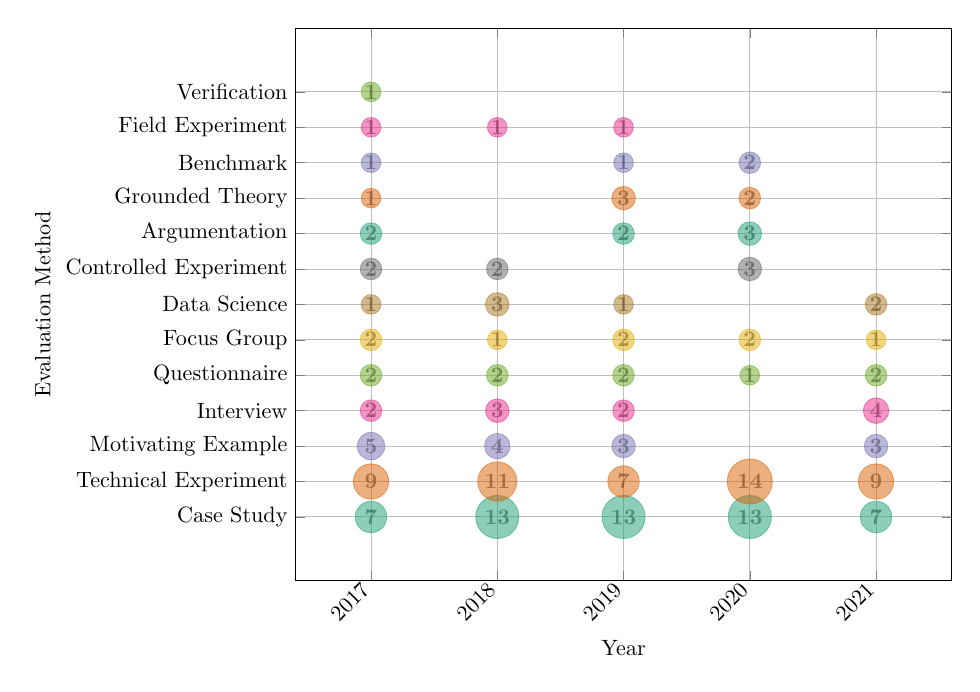
\begin{tikzpicture}[scale=.8]
\pgfplotsset{cycle list/Dark2}
\begin{axis}[width=.99\linewidth,
    enlargelimits=0.15,
    x tick label style={rotate=45,anchor=east},
    xtick={0,1,2,3,4}, xticklabels={2017,2018,2019,2020,2021},
    xlabel={Year},
    ytick={0,1,2,3,4,5,6,7,8,9,10,11,12}, yticklabels={Case Study,Technical Experiment,Motivating Example,Interview,Questionnaire,Focus Group,Data Science,Controlled Experiment,Argumentation,Grounded Theory,Benchmark,Field Experiment,Verification},
    ylabel={Evaluation Method},
    grid=both,
    scatter,scatter src=y,
    scatter/classes={0={draw=Dark2-A,fill=Dark2-A}, 1={draw=Dark2-B,fill=Dark2-B}, 2={draw=Dark2-C,fill=Dark2-C}, 3={draw=Dark2-D,fill=Dark2-D}, 4={draw=Dark2-E,fill=Dark2-E}, 5={draw=Dark2-F,fill=Dark2-F}, 6={draw=Dark2-G,fill=Dark2-G}, 7={draw=Dark2-H,fill=Dark2-H}, 8={draw=Dark2-A,fill=Dark2-A}, 9={draw=Dark2-B,fill=Dark2-B}, 10={draw=Dark2-C,fill=Dark2-C}, 11={draw=Dark2-D,fill=Dark2-D}, 12={draw=Dark2-E,fill=Dark2-E}}
]

\addplot+[mark=*,mark size=7.094,opacity=0.5,text=black] coordinates { (0,0) } node[text=black,font=\bfseries] {7};
\addplot+[mark=*,mark size=7.978,opacity=0.5,text=black] coordinates { (0,1) } node[text=black,font=\bfseries] {9};
\addplot+[mark=*,mark size=6.210,opacity=0.5,text=black] coordinates { (0,2) } node[text=black,font=\bfseries] {5};
\addplot+[mark=*,mark size=4.884,opacity=0.5,text=black] coordinates { (0,3) } node[text=black,font=\bfseries] {2};
\addplot+[mark=*,mark size=4.884,opacity=0.5,text=black] coordinates { (0,4) } node[text=black,font=\bfseries] {2};
\addplot+[mark=*,mark size=4.884,opacity=0.5,text=black] coordinates { (0,5) } node[text=black,font=\bfseries] {2};
\addplot+[mark=*,mark size=4.442,opacity=0.5,text=black] coordinates { (0,6) } node[text=black,font=\bfseries] {1};
\addplot+[mark=*,mark size=4.884,opacity=0.5,text=black] coordinates { (0,7) } node[text=black,font=\bfseries] {2};
\addplot+[mark=*,mark size=4.884,opacity=0.5,text=black] coordinates { (0,8) } node[text=black,font=\bfseries] {2};
\addplot+[mark=*,mark size=4.442,opacity=0.5,text=black] coordinates { (0,9) } node[text=black,font=\bfseries] {1};
\addplot+[mark=*,mark size=4.442,opacity=0.5,text=black] coordinates { (0,10) } node[text=black,font=\bfseries] {1};
\addplot+[mark=*,mark size=4.442,opacity=0.5,text=black] coordinates { (0,11) } node[text=black,font=\bfseries] {1};
\addplot+[mark=*,mark size=4.442,opacity=0.5,text=black] coordinates { (0,12) } node[text=black,font=\bfseries] {1};
\addplot+[mark=*,mark size=9.746,opacity=0.5,text=black] coordinates { (1,0) } node[text=black,font=\bfseries] {13};
\addplot+[mark=*,mark size=8.862,opacity=0.5,text=black] coordinates { (1,1) } node[text=black,font=\bfseries] {11};
\addplot+[mark=*,mark size=5.768,opacity=0.5,text=black] coordinates { (1,2) } node[text=black,font=\bfseries] {4};
\addplot+[mark=*,mark size=5.326,opacity=0.5,text=black] coordinates { (1,3) } node[text=black,font=\bfseries] {3};
\addplot+[mark=*,mark size=4.884,opacity=0.5,text=black] coordinates { (1,4) } node[text=black,font=\bfseries] {2};
\addplot+[mark=*,mark size=4.442,opacity=0.5,text=black] coordinates { (1,5) } node[text=black,font=\bfseries] {1};
\addplot+[mark=*,mark size=5.326,opacity=0.5,text=black] coordinates { (1,6) } node[text=black,font=\bfseries] {3};
\addplot+[mark=*,mark size=4.884,opacity=0.5,text=black] coordinates { (1,7) } node[text=black,font=\bfseries] {2};
\addplot+[mark=*,mark size=4.442,opacity=0.5,text=black] coordinates { (1,11) } node[text=black,font=\bfseries] {1};
\addplot+[mark=*,mark size=9.746,opacity=0.5,text=black] coordinates { (2,0) } node[text=black,font=\bfseries] {13};
\addplot+[mark=*,mark size=7.094,opacity=0.5,text=black] coordinates { (2,1) } node[text=black,font=\bfseries] {7};
\addplot+[mark=*,mark size=5.326,opacity=0.5,text=black] coordinates { (2,2) } node[text=black,font=\bfseries] {3};
\addplot+[mark=*,mark size=4.884,opacity=0.5,text=black] coordinates { (2,3) } node[text=black,font=\bfseries] {2};
\addplot+[mark=*,mark size=4.884,opacity=0.5,text=black] coordinates { (2,4) } node[text=black,font=\bfseries] {2};
\addplot+[mark=*,mark size=4.884,opacity=0.5,text=black] coordinates { (2,5) } node[text=black,font=\bfseries] {2};
\addplot+[mark=*,mark size=4.442,opacity=0.5,text=black] coordinates { (2,6) } node[text=black,font=\bfseries] {1};
\addplot+[mark=*,mark size=4.884,opacity=0.5,text=black] coordinates { (2,8) } node[text=black,font=\bfseries] {2};
\addplot+[mark=*,mark size=5.326,opacity=0.5,text=black] coordinates { (2,9) } node[text=black,font=\bfseries] {3};
\addplot+[mark=*,mark size=4.442,opacity=0.5,text=black] coordinates { (2,10) } node[text=black,font=\bfseries] {1};
\addplot+[mark=*,mark size=4.442,opacity=0.5,text=black] coordinates { (2,11) } node[text=black,font=\bfseries] {1};
\addplot+[mark=*,mark size=9.746,opacity=0.5,text=black] coordinates { (3,0) } node[text=black,font=\bfseries] {13};
\addplot+[mark=*,mark size=10.188,opacity=0.5,text=black] coordinates { (3,1) } node[text=black,font=\bfseries] {14};
\addplot+[mark=*,mark size=4.442,opacity=0.5,text=black] coordinates { (3,4) } node[text=black,font=\bfseries] {1};
\addplot+[mark=*,mark size=4.884,opacity=0.5,text=black] coordinates { (3,5) } node[text=black,font=\bfseries] {2};
\addplot+[mark=*,mark size=5.326,opacity=0.5,text=black] coordinates { (3,7) } node[text=black,font=\bfseries] {3};
\addplot+[mark=*,mark size=5.326,opacity=0.5,text=black] coordinates { (3,8) } node[text=black,font=\bfseries] {3};
\addplot+[mark=*,mark size=4.884,opacity=0.5,text=black] coordinates { (3,9) } node[text=black,font=\bfseries] {2};
\addplot+[mark=*,mark size=4.884,opacity=0.5,text=black] coordinates { (3,10) } node[text=black,font=\bfseries] {2};
\addplot+[mark=*,mark size=7.094,opacity=0.5,text=black] coordinates { (4,0) } node[text=black,font=\bfseries] {7};
\addplot+[mark=*,mark size=7.978,opacity=0.5,text=black] coordinates { (4,1) } node[text=black,font=\bfseries] {9};
\addplot+[mark=*,mark size=5.326,opacity=0.5,text=black] coordinates { (4,2) } node[text=black,font=\bfseries] {3};
\addplot+[mark=*,mark size=5.768,opacity=0.5,text=black] coordinates { (4,3) } node[text=black,font=\bfseries] {4};
\addplot+[mark=*,mark size=4.884,opacity=0.5,text=black] coordinates { (4,4) } node[text=black,font=\bfseries] {2};
\addplot+[mark=*,mark size=4.442,opacity=0.5,text=black] coordinates { (4,5) } node[text=black,font=\bfseries] {1};
\addplot+[mark=*,mark size=4.884,opacity=0.5,text=black] coordinates { (4,6) } node[text=black,font=\bfseries] {2};


\end{axis}
\end{tikzpicture}
\end{center}
%\caption{Portfolio f\"ur Year und Evaluation Method (Gr\"o\ss{}e entspricht der Anzahl)}\label{fig:port_year_evaluationmethod}
%\end{figure}



\section{Number of publications featuring a replication package (packaged), providing links to available tools or input data (available), employed tools or input data (used), or none of the above (none) from 2017 to 2021}

\input{figs/chisto_year_artifacts}

\section{Relations between research objects of publications and properties investigated for evaluation}

%\subsection{Portfolio f\"ur Property und Research Object (Gr\"o\ss{}e entspricht der Anzahl)}
%\begin{figure}
\begin{center}
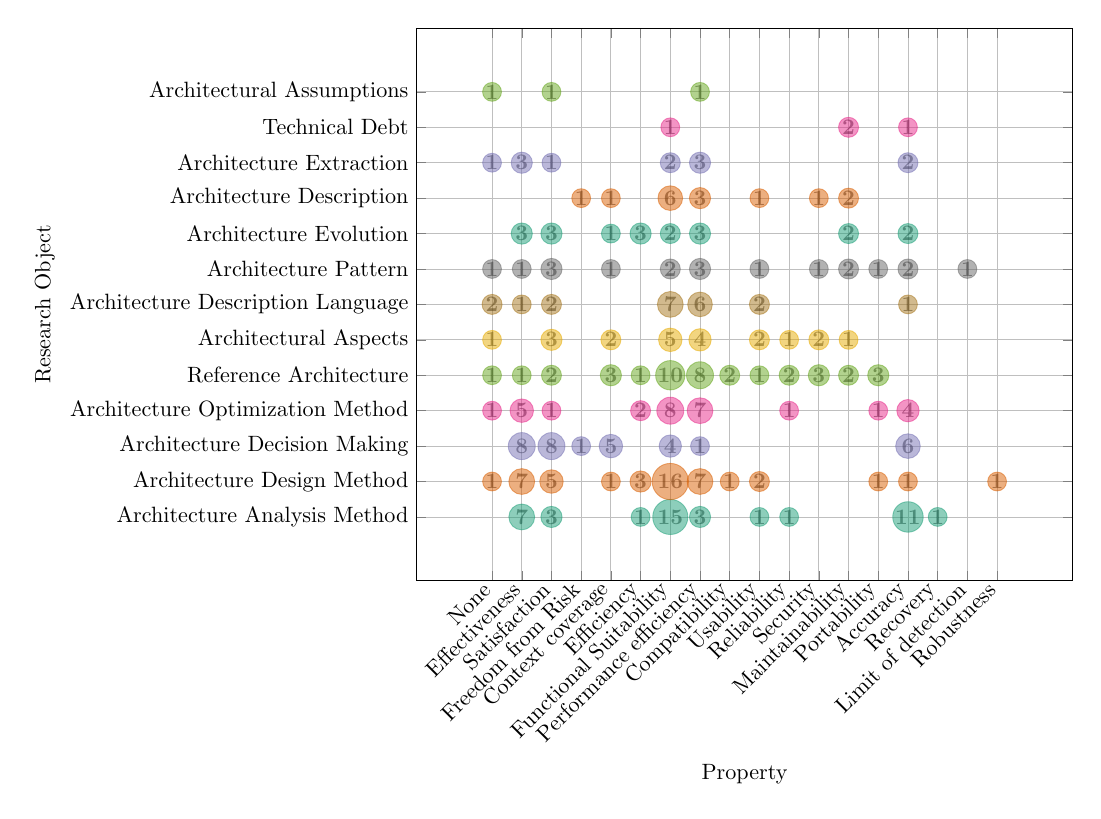
\begin{tikzpicture}[scale=.8]
\pgfplotsset{cycle list/Dark2}
\begin{axis}[width=.99\linewidth,
    enlargelimits=0.15,
    x tick label style={rotate=45,anchor=east},
    xtick={0,1,2,3,4,5,6,7,8,9,10,11,12,13,14,15,16,17}, xticklabels={None,Effectiveness,Satisfaction,Freedom from Risk,Context coverage,Efficiency,Functional Suitability,Performance efficiency,Compatibility,Usability,Reliability,Security,Maintainability,Portability,Accuracy,Recovery,Limit of detection,Robustness},
    xlabel={Property},
    ytick={0,1,2,3,4,5,6,7,8,9,10,11,12}, yticklabels={Architecture Analysis Method,Architecture Design Method,Architecture Decision Making,Architecture Optimization Method,Reference Architecture,Architectural Aspects,Architecture Description Language,Architecture Pattern,Architecture Evolution,Architecture Description,Architecture Extraction,Technical Debt,Architectural Assumptions},
    ylabel={Research Object},
    grid=both,
    scatter,scatter src=y,
    scatter/classes={0={draw=Dark2-A,fill=Dark2-A}, 1={draw=Dark2-B,fill=Dark2-B}, 2={draw=Dark2-C,fill=Dark2-C}, 3={draw=Dark2-D,fill=Dark2-D}, 4={draw=Dark2-E,fill=Dark2-E}, 5={draw=Dark2-F,fill=Dark2-F}, 6={draw=Dark2-G,fill=Dark2-G}, 7={draw=Dark2-H,fill=Dark2-H}, 8={draw=Dark2-A,fill=Dark2-A}, 9={draw=Dark2-B,fill=Dark2-B}, 10={draw=Dark2-C,fill=Dark2-C}, 11={draw=Dark2-D,fill=Dark2-D}, 12={draw=Dark2-E,fill=Dark2-E}}
]

\addplot+[mark=*,mark size=4.262,opacity=0.5,text=black] coordinates { (0,1) } node[text=black,font=\bfseries] {1};
\addplot+[mark=*,mark size=4.262,opacity=0.5,text=black] coordinates { (0,3) } node[text=black,font=\bfseries] {1};
\addplot+[mark=*,mark size=4.262,opacity=0.5,text=black] coordinates { (0,4) } node[text=black,font=\bfseries] {1};
\addplot+[mark=*,mark size=4.262,opacity=0.5,text=black] coordinates { (0,5) } node[text=black,font=\bfseries] {1};
\addplot+[mark=*,mark size=4.525,opacity=0.5,text=black] coordinates { (0,6) } node[text=black,font=\bfseries] {2};
\addplot+[mark=*,mark size=4.262,opacity=0.5,text=black] coordinates { (0,7) } node[text=black,font=\bfseries] {1};
\addplot+[mark=*,mark size=4.262,opacity=0.5,text=black] coordinates { (0,10) } node[text=black,font=\bfseries] {1};
\addplot+[mark=*,mark size=4.262,opacity=0.5,text=black] coordinates { (0,12) } node[text=black,font=\bfseries] {1};
\addplot+[mark=*,mark size=5.836,opacity=0.5,text=black] coordinates { (1,0) } node[text=black,font=\bfseries] {7};
\addplot+[mark=*,mark size=5.836,opacity=0.5,text=black] coordinates { (1,1) } node[text=black,font=\bfseries] {7};
\addplot+[mark=*,mark size=6.098,opacity=0.5,text=black] coordinates { (1,2) } node[text=black,font=\bfseries] {8};
\addplot+[mark=*,mark size=5.311,opacity=0.5,text=black] coordinates { (1,3) } node[text=black,font=\bfseries] {5};
\addplot+[mark=*,mark size=4.262,opacity=0.5,text=black] coordinates { (1,4) } node[text=black,font=\bfseries] {1};
\addplot+[mark=*,mark size=4.262,opacity=0.5,text=black] coordinates { (1,6) } node[text=black,font=\bfseries] {1};
\addplot+[mark=*,mark size=4.262,opacity=0.5,text=black] coordinates { (1,7) } node[text=black,font=\bfseries] {1};
\addplot+[mark=*,mark size=4.787,opacity=0.5,text=black] coordinates { (1,8) } node[text=black,font=\bfseries] {3};
\addplot+[mark=*,mark size=4.787,opacity=0.5,text=black] coordinates { (1,10) } node[text=black,font=\bfseries] {3};
\addplot+[mark=*,mark size=4.787,opacity=0.5,text=black] coordinates { (2,0) } node[text=black,font=\bfseries] {3};
\addplot+[mark=*,mark size=5.311,opacity=0.5,text=black] coordinates { (2,1) } node[text=black,font=\bfseries] {5};
\addplot+[mark=*,mark size=6.098,opacity=0.5,text=black] coordinates { (2,2) } node[text=black,font=\bfseries] {8};
\addplot+[mark=*,mark size=4.262,opacity=0.5,text=black] coordinates { (2,3) } node[text=black,font=\bfseries] {1};
\addplot+[mark=*,mark size=4.525,opacity=0.5,text=black] coordinates { (2,4) } node[text=black,font=\bfseries] {2};
\addplot+[mark=*,mark size=4.787,opacity=0.5,text=black] coordinates { (2,5) } node[text=black,font=\bfseries] {3};
\addplot+[mark=*,mark size=4.525,opacity=0.5,text=black] coordinates { (2,6) } node[text=black,font=\bfseries] {2};
\addplot+[mark=*,mark size=4.787,opacity=0.5,text=black] coordinates { (2,7) } node[text=black,font=\bfseries] {3};
\addplot+[mark=*,mark size=4.787,opacity=0.5,text=black] coordinates { (2,8) } node[text=black,font=\bfseries] {3};
\addplot+[mark=*,mark size=4.262,opacity=0.5,text=black] coordinates { (2,10) } node[text=black,font=\bfseries] {1};
\addplot+[mark=*,mark size=4.262,opacity=0.5,text=black] coordinates { (2,12) } node[text=black,font=\bfseries] {1};
\addplot+[mark=*,mark size=4.262,opacity=0.5,text=black] coordinates { (3,2) } node[text=black,font=\bfseries] {1};
\addplot+[mark=*,mark size=4.262,opacity=0.5,text=black] coordinates { (3,9) } node[text=black,font=\bfseries] {1};
\addplot+[mark=*,mark size=4.262,opacity=0.5,text=black] coordinates { (4,1) } node[text=black,font=\bfseries] {1};
\addplot+[mark=*,mark size=5.311,opacity=0.5,text=black] coordinates { (4,2) } node[text=black,font=\bfseries] {5};
\addplot+[mark=*,mark size=4.787,opacity=0.5,text=black] coordinates { (4,4) } node[text=black,font=\bfseries] {3};
\addplot+[mark=*,mark size=4.525,opacity=0.5,text=black] coordinates { (4,5) } node[text=black,font=\bfseries] {2};
\addplot+[mark=*,mark size=4.262,opacity=0.5,text=black] coordinates { (4,7) } node[text=black,font=\bfseries] {1};
\addplot+[mark=*,mark size=4.262,opacity=0.5,text=black] coordinates { (4,8) } node[text=black,font=\bfseries] {1};
\addplot+[mark=*,mark size=4.262,opacity=0.5,text=black] coordinates { (4,9) } node[text=black,font=\bfseries] {1};
\addplot+[mark=*,mark size=4.262,opacity=0.5,text=black] coordinates { (5,0) } node[text=black,font=\bfseries] {1};
\addplot+[mark=*,mark size=4.787,opacity=0.5,text=black] coordinates { (5,1) } node[text=black,font=\bfseries] {3};
\addplot+[mark=*,mark size=4.525,opacity=0.5,text=black] coordinates { (5,3) } node[text=black,font=\bfseries] {2};
\addplot+[mark=*,mark size=4.262,opacity=0.5,text=black] coordinates { (5,4) } node[text=black,font=\bfseries] {1};
\addplot+[mark=*,mark size=4.787,opacity=0.5,text=black] coordinates { (5,8) } node[text=black,font=\bfseries] {3};
\addplot+[mark=*,mark size=7.934,opacity=0.5,text=black] coordinates { (6,0) } node[text=black,font=\bfseries] {15};
\addplot+[mark=*,mark size=8.197,opacity=0.5,text=black] coordinates { (6,1) } node[text=black,font=\bfseries] {16};
\addplot+[mark=*,mark size=5.049,opacity=0.5,text=black] coordinates { (6,2) } node[text=black,font=\bfseries] {4};
\addplot+[mark=*,mark size=6.098,opacity=0.5,text=black] coordinates { (6,3) } node[text=black,font=\bfseries] {8};
\addplot+[mark=*,mark size=6.623,opacity=0.5,text=black] coordinates { (6,4) } node[text=black,font=\bfseries] {10};
\addplot+[mark=*,mark size=5.311,opacity=0.5,text=black] coordinates { (6,5) } node[text=black,font=\bfseries] {5};
\addplot+[mark=*,mark size=5.836,opacity=0.5,text=black] coordinates { (6,6) } node[text=black,font=\bfseries] {7};
\addplot+[mark=*,mark size=4.525,opacity=0.5,text=black] coordinates { (6,7) } node[text=black,font=\bfseries] {2};
\addplot+[mark=*,mark size=4.525,opacity=0.5,text=black] coordinates { (6,8) } node[text=black,font=\bfseries] {2};
\addplot+[mark=*,mark size=5.574,opacity=0.5,text=black] coordinates { (6,9) } node[text=black,font=\bfseries] {6};
\addplot+[mark=*,mark size=4.525,opacity=0.5,text=black] coordinates { (6,10) } node[text=black,font=\bfseries] {2};
\addplot+[mark=*,mark size=4.262,opacity=0.5,text=black] coordinates { (6,11) } node[text=black,font=\bfseries] {1};
\addplot+[mark=*,mark size=4.787,opacity=0.5,text=black] coordinates { (7,0) } node[text=black,font=\bfseries] {3};
\addplot+[mark=*,mark size=5.836,opacity=0.5,text=black] coordinates { (7,1) } node[text=black,font=\bfseries] {7};
\addplot+[mark=*,mark size=4.262,opacity=0.5,text=black] coordinates { (7,2) } node[text=black,font=\bfseries] {1};
\addplot+[mark=*,mark size=5.836,opacity=0.5,text=black] coordinates { (7,3) } node[text=black,font=\bfseries] {7};
\addplot+[mark=*,mark size=6.098,opacity=0.5,text=black] coordinates { (7,4) } node[text=black,font=\bfseries] {8};
\addplot+[mark=*,mark size=5.049,opacity=0.5,text=black] coordinates { (7,5) } node[text=black,font=\bfseries] {4};
\addplot+[mark=*,mark size=5.574,opacity=0.5,text=black] coordinates { (7,6) } node[text=black,font=\bfseries] {6};
\addplot+[mark=*,mark size=4.787,opacity=0.5,text=black] coordinates { (7,7) } node[text=black,font=\bfseries] {3};
\addplot+[mark=*,mark size=4.787,opacity=0.5,text=black] coordinates { (7,8) } node[text=black,font=\bfseries] {3};
\addplot+[mark=*,mark size=4.787,opacity=0.5,text=black] coordinates { (7,9) } node[text=black,font=\bfseries] {3};
\addplot+[mark=*,mark size=4.787,opacity=0.5,text=black] coordinates { (7,10) } node[text=black,font=\bfseries] {3};
\addplot+[mark=*,mark size=4.262,opacity=0.5,text=black] coordinates { (7,12) } node[text=black,font=\bfseries] {1};
\addplot+[mark=*,mark size=4.262,opacity=0.5,text=black] coordinates { (8,1) } node[text=black,font=\bfseries] {1};
\addplot+[mark=*,mark size=4.525,opacity=0.5,text=black] coordinates { (8,4) } node[text=black,font=\bfseries] {2};
\addplot+[mark=*,mark size=4.262,opacity=0.5,text=black] coordinates { (9,0) } node[text=black,font=\bfseries] {1};
\addplot+[mark=*,mark size=4.525,opacity=0.5,text=black] coordinates { (9,1) } node[text=black,font=\bfseries] {2};
\addplot+[mark=*,mark size=4.262,opacity=0.5,text=black] coordinates { (9,4) } node[text=black,font=\bfseries] {1};
\addplot+[mark=*,mark size=4.525,opacity=0.5,text=black] coordinates { (9,5) } node[text=black,font=\bfseries] {2};
\addplot+[mark=*,mark size=4.525,opacity=0.5,text=black] coordinates { (9,6) } node[text=black,font=\bfseries] {2};
\addplot+[mark=*,mark size=4.262,opacity=0.5,text=black] coordinates { (9,7) } node[text=black,font=\bfseries] {1};
\addplot+[mark=*,mark size=4.262,opacity=0.5,text=black] coordinates { (9,9) } node[text=black,font=\bfseries] {1};
\addplot+[mark=*,mark size=4.262,opacity=0.5,text=black] coordinates { (10,0) } node[text=black,font=\bfseries] {1};
\addplot+[mark=*,mark size=4.262,opacity=0.5,text=black] coordinates { (10,3) } node[text=black,font=\bfseries] {1};
\addplot+[mark=*,mark size=4.525,opacity=0.5,text=black] coordinates { (10,4) } node[text=black,font=\bfseries] {2};
\addplot+[mark=*,mark size=4.262,opacity=0.5,text=black] coordinates { (10,5) } node[text=black,font=\bfseries] {1};
\addplot+[mark=*,mark size=4.787,opacity=0.5,text=black] coordinates { (11,4) } node[text=black,font=\bfseries] {3};
\addplot+[mark=*,mark size=4.525,opacity=0.5,text=black] coordinates { (11,5) } node[text=black,font=\bfseries] {2};
\addplot+[mark=*,mark size=4.262,opacity=0.5,text=black] coordinates { (11,7) } node[text=black,font=\bfseries] {1};
\addplot+[mark=*,mark size=4.262,opacity=0.5,text=black] coordinates { (11,9) } node[text=black,font=\bfseries] {1};
\addplot+[mark=*,mark size=4.525,opacity=0.5,text=black] coordinates { (12,4) } node[text=black,font=\bfseries] {2};
\addplot+[mark=*,mark size=4.262,opacity=0.5,text=black] coordinates { (12,5) } node[text=black,font=\bfseries] {1};
\addplot+[mark=*,mark size=4.525,opacity=0.5,text=black] coordinates { (12,7) } node[text=black,font=\bfseries] {2};
\addplot+[mark=*,mark size=4.525,opacity=0.5,text=black] coordinates { (12,8) } node[text=black,font=\bfseries] {2};
\addplot+[mark=*,mark size=4.525,opacity=0.5,text=black] coordinates { (12,9) } node[text=black,font=\bfseries] {2};
\addplot+[mark=*,mark size=4.525,opacity=0.5,text=black] coordinates { (12,11) } node[text=black,font=\bfseries] {2};
\addplot+[mark=*,mark size=4.262,opacity=0.5,text=black] coordinates { (13,1) } node[text=black,font=\bfseries] {1};
\addplot+[mark=*,mark size=4.262,opacity=0.5,text=black] coordinates { (13,3) } node[text=black,font=\bfseries] {1};
\addplot+[mark=*,mark size=4.787,opacity=0.5,text=black] coordinates { (13,4) } node[text=black,font=\bfseries] {3};
\addplot+[mark=*,mark size=4.262,opacity=0.5,text=black] coordinates { (13,7) } node[text=black,font=\bfseries] {1};
\addplot+[mark=*,mark size=6.885,opacity=0.5,text=black] coordinates { (14,0) } node[text=black,font=\bfseries] {11};
\addplot+[mark=*,mark size=4.262,opacity=0.5,text=black] coordinates { (14,1) } node[text=black,font=\bfseries] {1};
\addplot+[mark=*,mark size=5.574,opacity=0.5,text=black] coordinates { (14,2) } node[text=black,font=\bfseries] {6};
\addplot+[mark=*,mark size=5.049,opacity=0.5,text=black] coordinates { (14,3) } node[text=black,font=\bfseries] {4};
\addplot+[mark=*,mark size=4.262,opacity=0.5,text=black] coordinates { (14,6) } node[text=black,font=\bfseries] {1};
\addplot+[mark=*,mark size=4.525,opacity=0.5,text=black] coordinates { (14,7) } node[text=black,font=\bfseries] {2};
\addplot+[mark=*,mark size=4.525,opacity=0.5,text=black] coordinates { (14,8) } node[text=black,font=\bfseries] {2};
\addplot+[mark=*,mark size=4.525,opacity=0.5,text=black] coordinates { (14,10) } node[text=black,font=\bfseries] {2};
\addplot+[mark=*,mark size=4.262,opacity=0.5,text=black] coordinates { (14,11) } node[text=black,font=\bfseries] {1};
\addplot+[mark=*,mark size=4.262,opacity=0.5,text=black] coordinates { (15,0) } node[text=black,font=\bfseries] {1};
\addplot+[mark=*,mark size=4.262,opacity=0.5,text=black] coordinates { (16,7) } node[text=black,font=\bfseries] {1};
\addplot+[mark=*,mark size=4.262,opacity=0.5,text=black] coordinates { (17,1) } node[text=black,font=\bfseries] {1};


\end{axis}
\end{tikzpicture}
\end{center}
%\caption{Portfolio f\"ur Property und Research Object (Gr\"o\ss{}e entspricht der Anzahl)}\label{fig:port_property_researchobject}
%\end{figure}



\section{Relations between research objects of publications and evaluation methods applied}

%\subsection{Portfolio f\"ur Evaluation Method und Research Object (Gr\"o\ss{}e entspricht der Anzahl)}
%\begin{figure}
\begin{center}
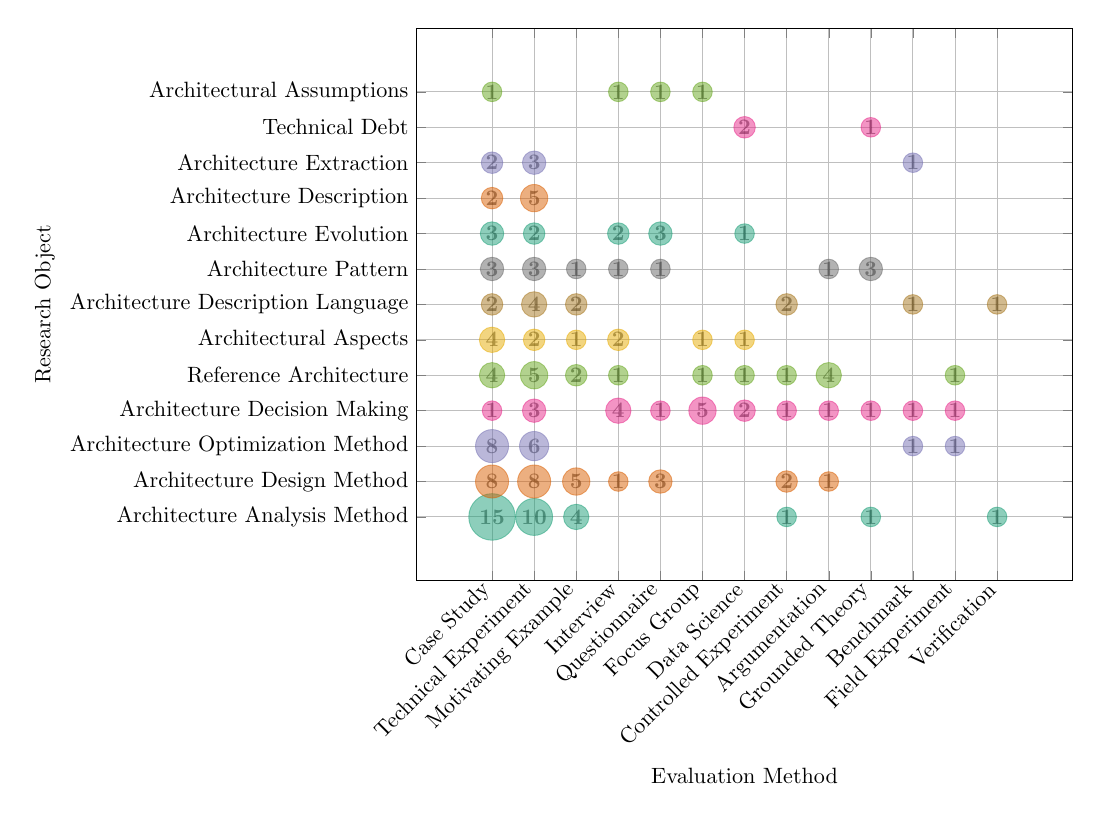
\begin{tikzpicture}[scale=.8]
\pgfplotsset{cycle list/Dark2}
\begin{axis}[width=.99\linewidth,
    enlargelimits=0.15,
    x tick label style={rotate=45,anchor=east},
    xtick={0,1,2,3,4,5,6,7,8,9,10,11,12}, xticklabels={Case Study,Technical Experiment,Motivating Example,Interview,Questionnaire,Focus Group,Data Science,Controlled Experiment,Argumentation,Grounded Theory,Benchmark,Field Experiment,Verification},
    xlabel={Evaluation Method},
    ytick={0,1,2,3,4,5,6,7,8,9,10,11,12}, yticklabels={Architecture Analysis Method,Architecture Design Method,Architecture Optimization Method,Architecture Decision Making,Reference Architecture,Architectural Aspects,Architecture Description Language,Architecture Pattern,Architecture Evolution,Architecture Description,Architecture Extraction,Technical Debt,Architectural Assumptions},
    ylabel={Research Object},
    grid=both,
    scatter,scatter src=y,
    scatter/classes={0={draw=Dark2-A,fill=Dark2-A}, 1={draw=Dark2-B,fill=Dark2-B}, 2={draw=Dark2-C,fill=Dark2-C}, 3={draw=Dark2-D,fill=Dark2-D}, 4={draw=Dark2-E,fill=Dark2-E}, 5={draw=Dark2-F,fill=Dark2-F}, 6={draw=Dark2-G,fill=Dark2-G}, 7={draw=Dark2-H,fill=Dark2-H}, 8={draw=Dark2-A,fill=Dark2-A}, 9={draw=Dark2-B,fill=Dark2-B}, 10={draw=Dark2-C,fill=Dark2-C}, 11={draw=Dark2-D,fill=Dark2-D}, 12={draw=Dark2-E,fill=Dark2-E}}
]

\addplot+[mark=*,mark size=10.522,opacity=0.5,text=black] coordinates { (0,0) } node[text=black,font=\bfseries] {15};
\addplot+[mark=*,mark size=7.478,opacity=0.5,text=black] coordinates { (0,1) } node[text=black,font=\bfseries] {8};
\addplot+[mark=*,mark size=7.478,opacity=0.5,text=black] coordinates { (0,2) } node[text=black,font=\bfseries] {8};
\addplot+[mark=*,mark size=4.435,opacity=0.5,text=black] coordinates { (0,3) } node[text=black,font=\bfseries] {1};
\addplot+[mark=*,mark size=5.739,opacity=0.5,text=black] coordinates { (0,4) } node[text=black,font=\bfseries] {4};
\addplot+[mark=*,mark size=5.739,opacity=0.5,text=black] coordinates { (0,5) } node[text=black,font=\bfseries] {4};
\addplot+[mark=*,mark size=4.870,opacity=0.5,text=black] coordinates { (0,6) } node[text=black,font=\bfseries] {2};
\addplot+[mark=*,mark size=5.304,opacity=0.5,text=black] coordinates { (0,7) } node[text=black,font=\bfseries] {3};
\addplot+[mark=*,mark size=5.304,opacity=0.5,text=black] coordinates { (0,8) } node[text=black,font=\bfseries] {3};
\addplot+[mark=*,mark size=4.870,opacity=0.5,text=black] coordinates { (0,9) } node[text=black,font=\bfseries] {2};
\addplot+[mark=*,mark size=4.870,opacity=0.5,text=black] coordinates { (0,10) } node[text=black,font=\bfseries] {2};
\addplot+[mark=*,mark size=4.435,opacity=0.5,text=black] coordinates { (0,12) } node[text=black,font=\bfseries] {1};
\addplot+[mark=*,mark size=8.348,opacity=0.5,text=black] coordinates { (1,0) } node[text=black,font=\bfseries] {10};
\addplot+[mark=*,mark size=7.478,opacity=0.5,text=black] coordinates { (1,1) } node[text=black,font=\bfseries] {8};
\addplot+[mark=*,mark size=6.609,opacity=0.5,text=black] coordinates { (1,2) } node[text=black,font=\bfseries] {6};
\addplot+[mark=*,mark size=5.304,opacity=0.5,text=black] coordinates { (1,3) } node[text=black,font=\bfseries] {3};
\addplot+[mark=*,mark size=6.174,opacity=0.5,text=black] coordinates { (1,4) } node[text=black,font=\bfseries] {5};
\addplot+[mark=*,mark size=4.870,opacity=0.5,text=black] coordinates { (1,5) } node[text=black,font=\bfseries] {2};
\addplot+[mark=*,mark size=5.739,opacity=0.5,text=black] coordinates { (1,6) } node[text=black,font=\bfseries] {4};
\addplot+[mark=*,mark size=5.304,opacity=0.5,text=black] coordinates { (1,7) } node[text=black,font=\bfseries] {3};
\addplot+[mark=*,mark size=4.870,opacity=0.5,text=black] coordinates { (1,8) } node[text=black,font=\bfseries] {2};
\addplot+[mark=*,mark size=6.174,opacity=0.5,text=black] coordinates { (1,9) } node[text=black,font=\bfseries] {5};
\addplot+[mark=*,mark size=5.304,opacity=0.5,text=black] coordinates { (1,10) } node[text=black,font=\bfseries] {3};
\addplot+[mark=*,mark size=5.739,opacity=0.5,text=black] coordinates { (2,0) } node[text=black,font=\bfseries] {4};
\addplot+[mark=*,mark size=6.174,opacity=0.5,text=black] coordinates { (2,1) } node[text=black,font=\bfseries] {5};
\addplot+[mark=*,mark size=4.870,opacity=0.5,text=black] coordinates { (2,4) } node[text=black,font=\bfseries] {2};
\addplot+[mark=*,mark size=4.435,opacity=0.5,text=black] coordinates { (2,5) } node[text=black,font=\bfseries] {1};
\addplot+[mark=*,mark size=4.870,opacity=0.5,text=black] coordinates { (2,6) } node[text=black,font=\bfseries] {2};
\addplot+[mark=*,mark size=4.435,opacity=0.5,text=black] coordinates { (2,7) } node[text=black,font=\bfseries] {1};
\addplot+[mark=*,mark size=4.435,opacity=0.5,text=black] coordinates { (3,1) } node[text=black,font=\bfseries] {1};
\addplot+[mark=*,mark size=5.739,opacity=0.5,text=black] coordinates { (3,3) } node[text=black,font=\bfseries] {4};
\addplot+[mark=*,mark size=4.435,opacity=0.5,text=black] coordinates { (3,4) } node[text=black,font=\bfseries] {1};
\addplot+[mark=*,mark size=4.870,opacity=0.5,text=black] coordinates { (3,5) } node[text=black,font=\bfseries] {2};
\addplot+[mark=*,mark size=4.435,opacity=0.5,text=black] coordinates { (3,7) } node[text=black,font=\bfseries] {1};
\addplot+[mark=*,mark size=4.870,opacity=0.5,text=black] coordinates { (3,8) } node[text=black,font=\bfseries] {2};
\addplot+[mark=*,mark size=4.435,opacity=0.5,text=black] coordinates { (3,12) } node[text=black,font=\bfseries] {1};
\addplot+[mark=*,mark size=5.304,opacity=0.5,text=black] coordinates { (4,1) } node[text=black,font=\bfseries] {3};
\addplot+[mark=*,mark size=4.435,opacity=0.5,text=black] coordinates { (4,3) } node[text=black,font=\bfseries] {1};
\addplot+[mark=*,mark size=4.435,opacity=0.5,text=black] coordinates { (4,7) } node[text=black,font=\bfseries] {1};
\addplot+[mark=*,mark size=5.304,opacity=0.5,text=black] coordinates { (4,8) } node[text=black,font=\bfseries] {3};
\addplot+[mark=*,mark size=4.435,opacity=0.5,text=black] coordinates { (4,12) } node[text=black,font=\bfseries] {1};
\addplot+[mark=*,mark size=6.174,opacity=0.5,text=black] coordinates { (5,3) } node[text=black,font=\bfseries] {5};
\addplot+[mark=*,mark size=4.435,opacity=0.5,text=black] coordinates { (5,4) } node[text=black,font=\bfseries] {1};
\addplot+[mark=*,mark size=4.435,opacity=0.5,text=black] coordinates { (5,5) } node[text=black,font=\bfseries] {1};
\addplot+[mark=*,mark size=4.435,opacity=0.5,text=black] coordinates { (5,12) } node[text=black,font=\bfseries] {1};
\addplot+[mark=*,mark size=4.870,opacity=0.5,text=black] coordinates { (6,3) } node[text=black,font=\bfseries] {2};
\addplot+[mark=*,mark size=4.435,opacity=0.5,text=black] coordinates { (6,4) } node[text=black,font=\bfseries] {1};
\addplot+[mark=*,mark size=4.435,opacity=0.5,text=black] coordinates { (6,5) } node[text=black,font=\bfseries] {1};
\addplot+[mark=*,mark size=4.435,opacity=0.5,text=black] coordinates { (6,8) } node[text=black,font=\bfseries] {1};
\addplot+[mark=*,mark size=4.870,opacity=0.5,text=black] coordinates { (6,11) } node[text=black,font=\bfseries] {2};
\addplot+[mark=*,mark size=4.435,opacity=0.5,text=black] coordinates { (7,0) } node[text=black,font=\bfseries] {1};
\addplot+[mark=*,mark size=4.870,opacity=0.5,text=black] coordinates { (7,1) } node[text=black,font=\bfseries] {2};
\addplot+[mark=*,mark size=4.435,opacity=0.5,text=black] coordinates { (7,3) } node[text=black,font=\bfseries] {1};
\addplot+[mark=*,mark size=4.435,opacity=0.5,text=black] coordinates { (7,4) } node[text=black,font=\bfseries] {1};
\addplot+[mark=*,mark size=4.870,opacity=0.5,text=black] coordinates { (7,6) } node[text=black,font=\bfseries] {2};
\addplot+[mark=*,mark size=4.435,opacity=0.5,text=black] coordinates { (8,1) } node[text=black,font=\bfseries] {1};
\addplot+[mark=*,mark size=4.435,opacity=0.5,text=black] coordinates { (8,3) } node[text=black,font=\bfseries] {1};
\addplot+[mark=*,mark size=5.739,opacity=0.5,text=black] coordinates { (8,4) } node[text=black,font=\bfseries] {4};
\addplot+[mark=*,mark size=4.435,opacity=0.5,text=black] coordinates { (8,7) } node[text=black,font=\bfseries] {1};
\addplot+[mark=*,mark size=4.435,opacity=0.5,text=black] coordinates { (9,0) } node[text=black,font=\bfseries] {1};
\addplot+[mark=*,mark size=4.435,opacity=0.5,text=black] coordinates { (9,3) } node[text=black,font=\bfseries] {1};
\addplot+[mark=*,mark size=5.304,opacity=0.5,text=black] coordinates { (9,7) } node[text=black,font=\bfseries] {3};
\addplot+[mark=*,mark size=4.435,opacity=0.5,text=black] coordinates { (9,11) } node[text=black,font=\bfseries] {1};
\addplot+[mark=*,mark size=4.435,opacity=0.5,text=black] coordinates { (10,2) } node[text=black,font=\bfseries] {1};
\addplot+[mark=*,mark size=4.435,opacity=0.5,text=black] coordinates { (10,3) } node[text=black,font=\bfseries] {1};
\addplot+[mark=*,mark size=4.435,opacity=0.5,text=black] coordinates { (10,6) } node[text=black,font=\bfseries] {1};
\addplot+[mark=*,mark size=4.435,opacity=0.5,text=black] coordinates { (10,10) } node[text=black,font=\bfseries] {1};
\addplot+[mark=*,mark size=4.435,opacity=0.5,text=black] coordinates { (11,2) } node[text=black,font=\bfseries] {1};
\addplot+[mark=*,mark size=4.435,opacity=0.5,text=black] coordinates { (11,3) } node[text=black,font=\bfseries] {1};
\addplot+[mark=*,mark size=4.435,opacity=0.5,text=black] coordinates { (11,4) } node[text=black,font=\bfseries] {1};
\addplot+[mark=*,mark size=4.435,opacity=0.5,text=black] coordinates { (12,0) } node[text=black,font=\bfseries] {1};
\addplot+[mark=*,mark size=4.435,opacity=0.5,text=black] coordinates { (12,6) } node[text=black,font=\bfseries] {1};


\end{axis}
\end{tikzpicture}
\end{center}
%\caption{Portfolio f\"ur Evaluation Method und Research Object (Gr\"o\ss{}e entspricht der Anzahl)}\label{fig:port_evaluationmethod_researchobject}
%\end{figure}



\section{Relations between evaluation methods (per research object) and evaluated property}

%\subsection{Portfolio f\"ur Property und Evaluation Method (Gr\"o\ss{}e entspricht der Anzahl)}
%\begin{figure}
\begin{center}
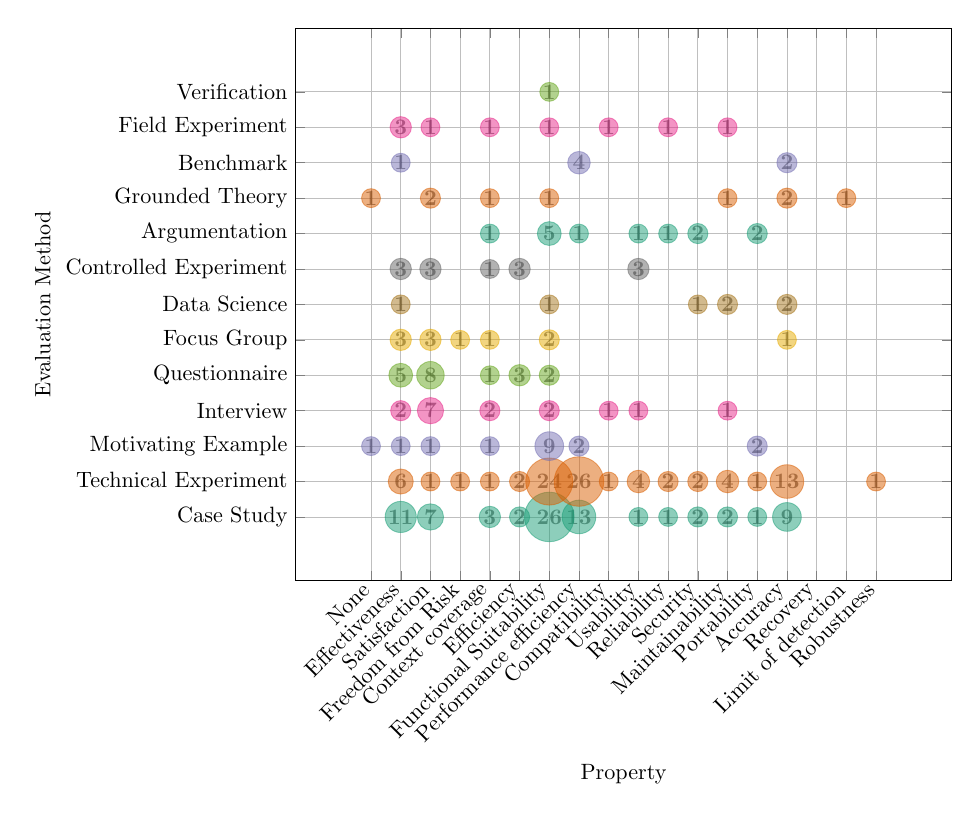
\begin{tikzpicture}[scale=.8]
\pgfplotsset{cycle list/Dark2}
\begin{axis}[width=.99\linewidth,
    enlargelimits=0.15,
    x tick label style={rotate=45,anchor=east},
    xtick={0,1,2,3,4,5,6,7,8,9,10,11,12,13,14,15,16,17}, xticklabels={None,Effectiveness,Satisfaction,Freedom from Risk,Context coverage,Efficiency,Functional Suitability,Performance efficiency,Compatibility,Usability,Reliability,Security,Maintainability,Portability,Accuracy,Recovery,Limit of detection,Robustness},
    xlabel={Property},
    ytick={0,1,2,3,4,5,6,7,8,9,10,11,12}, yticklabels={Case Study,Technical Experiment,Motivating Example,Interview,Questionnaire,Focus Group,Data Science,Controlled Experiment,Argumentation,Grounded Theory,Benchmark,Field Experiment,Verification},
    ylabel={Evaluation Method},
    grid=both,
    scatter,scatter src=y,
    scatter/classes={0={draw=Dark2-A,fill=Dark2-A}, 1={draw=Dark2-B,fill=Dark2-B}, 2={draw=Dark2-C,fill=Dark2-C}, 3={draw=Dark2-D,fill=Dark2-D}, 4={draw=Dark2-E,fill=Dark2-E}, 5={draw=Dark2-F,fill=Dark2-F}, 6={draw=Dark2-G,fill=Dark2-G}, 7={draw=Dark2-H,fill=Dark2-H}, 8={draw=Dark2-A,fill=Dark2-A}, 9={draw=Dark2-B,fill=Dark2-B}, 10={draw=Dark2-C,fill=Dark2-C}, 11={draw=Dark2-D,fill=Dark2-D}, 12={draw=Dark2-E,fill=Dark2-E}}
]

\addplot+[mark=*,mark size=4.277,opacity=0.5,text=black] coordinates { (0,2) } node[text=black,font=\bfseries] {1};
\addplot+[mark=*,mark size=4.277,opacity=0.5,text=black] coordinates { (0,9) } node[text=black,font=\bfseries] {1};
\addplot+[mark=*,mark size=7.045,opacity=0.5,text=black] coordinates { (1,0) } node[text=black,font=\bfseries] {11};
\addplot+[mark=*,mark size=5.661,opacity=0.5,text=black] coordinates { (1,1) } node[text=black,font=\bfseries] {6};
\addplot+[mark=*,mark size=4.277,opacity=0.5,text=black] coordinates { (1,2) } node[text=black,font=\bfseries] {1};
\addplot+[mark=*,mark size=4.554,opacity=0.5,text=black] coordinates { (1,3) } node[text=black,font=\bfseries] {2};
\addplot+[mark=*,mark size=5.384,opacity=0.5,text=black] coordinates { (1,4) } node[text=black,font=\bfseries] {5};
\addplot+[mark=*,mark size=4.830,opacity=0.5,text=black] coordinates { (1,5) } node[text=black,font=\bfseries] {3};
\addplot+[mark=*,mark size=4.277,opacity=0.5,text=black] coordinates { (1,6) } node[text=black,font=\bfseries] {1};
\addplot+[mark=*,mark size=4.830,opacity=0.5,text=black] coordinates { (1,7) } node[text=black,font=\bfseries] {3};
\addplot+[mark=*,mark size=4.277,opacity=0.5,text=black] coordinates { (1,10) } node[text=black,font=\bfseries] {1};
\addplot+[mark=*,mark size=4.830,opacity=0.5,text=black] coordinates { (1,11) } node[text=black,font=\bfseries] {3};
\addplot+[mark=*,mark size=5.938,opacity=0.5,text=black] coordinates { (2,0) } node[text=black,font=\bfseries] {7};
\addplot+[mark=*,mark size=4.277,opacity=0.5,text=black] coordinates { (2,1) } node[text=black,font=\bfseries] {1};
\addplot+[mark=*,mark size=4.277,opacity=0.5,text=black] coordinates { (2,2) } node[text=black,font=\bfseries] {1};
\addplot+[mark=*,mark size=5.938,opacity=0.5,text=black] coordinates { (2,3) } node[text=black,font=\bfseries] {7};
\addplot+[mark=*,mark size=6.215,opacity=0.5,text=black] coordinates { (2,4) } node[text=black,font=\bfseries] {8};
\addplot+[mark=*,mark size=4.830,opacity=0.5,text=black] coordinates { (2,5) } node[text=black,font=\bfseries] {3};
\addplot+[mark=*,mark size=4.830,opacity=0.5,text=black] coordinates { (2,7) } node[text=black,font=\bfseries] {3};
\addplot+[mark=*,mark size=4.554,opacity=0.5,text=black] coordinates { (2,9) } node[text=black,font=\bfseries] {2};
\addplot+[mark=*,mark size=4.277,opacity=0.5,text=black] coordinates { (2,11) } node[text=black,font=\bfseries] {1};
\addplot+[mark=*,mark size=4.277,opacity=0.5,text=black] coordinates { (3,1) } node[text=black,font=\bfseries] {1};
\addplot+[mark=*,mark size=4.277,opacity=0.5,text=black] coordinates { (3,5) } node[text=black,font=\bfseries] {1};
\addplot+[mark=*,mark size=4.830,opacity=0.5,text=black] coordinates { (4,0) } node[text=black,font=\bfseries] {3};
\addplot+[mark=*,mark size=4.277,opacity=0.5,text=black] coordinates { (4,1) } node[text=black,font=\bfseries] {1};
\addplot+[mark=*,mark size=4.277,opacity=0.5,text=black] coordinates { (4,2) } node[text=black,font=\bfseries] {1};
\addplot+[mark=*,mark size=4.554,opacity=0.5,text=black] coordinates { (4,3) } node[text=black,font=\bfseries] {2};
\addplot+[mark=*,mark size=4.277,opacity=0.5,text=black] coordinates { (4,4) } node[text=black,font=\bfseries] {1};
\addplot+[mark=*,mark size=4.277,opacity=0.5,text=black] coordinates { (4,5) } node[text=black,font=\bfseries] {1};
\addplot+[mark=*,mark size=4.277,opacity=0.5,text=black] coordinates { (4,7) } node[text=black,font=\bfseries] {1};
\addplot+[mark=*,mark size=4.277,opacity=0.5,text=black] coordinates { (4,8) } node[text=black,font=\bfseries] {1};
\addplot+[mark=*,mark size=4.277,opacity=0.5,text=black] coordinates { (4,9) } node[text=black,font=\bfseries] {1};
\addplot+[mark=*,mark size=4.277,opacity=0.5,text=black] coordinates { (4,11) } node[text=black,font=\bfseries] {1};
\addplot+[mark=*,mark size=4.554,opacity=0.5,text=black] coordinates { (5,0) } node[text=black,font=\bfseries] {2};
\addplot+[mark=*,mark size=4.554,opacity=0.5,text=black] coordinates { (5,1) } node[text=black,font=\bfseries] {2};
\addplot+[mark=*,mark size=4.830,opacity=0.5,text=black] coordinates { (5,4) } node[text=black,font=\bfseries] {3};
\addplot+[mark=*,mark size=4.830,opacity=0.5,text=black] coordinates { (5,7) } node[text=black,font=\bfseries] {3};
\addplot+[mark=*,mark size=11.197,opacity=0.5,text=black] coordinates { (6,0) } node[text=black,font=\bfseries] {26};
\addplot+[mark=*,mark size=10.644,opacity=0.5,text=black] coordinates { (6,1) } node[text=black,font=\bfseries] {24};
\addplot+[mark=*,mark size=6.491,opacity=0.5,text=black] coordinates { (6,2) } node[text=black,font=\bfseries] {9};
\addplot+[mark=*,mark size=4.554,opacity=0.5,text=black] coordinates { (6,3) } node[text=black,font=\bfseries] {2};
\addplot+[mark=*,mark size=4.554,opacity=0.5,text=black] coordinates { (6,4) } node[text=black,font=\bfseries] {2};
\addplot+[mark=*,mark size=4.554,opacity=0.5,text=black] coordinates { (6,5) } node[text=black,font=\bfseries] {2};
\addplot+[mark=*,mark size=4.277,opacity=0.5,text=black] coordinates { (6,6) } node[text=black,font=\bfseries] {1};
\addplot+[mark=*,mark size=5.384,opacity=0.5,text=black] coordinates { (6,8) } node[text=black,font=\bfseries] {5};
\addplot+[mark=*,mark size=4.277,opacity=0.5,text=black] coordinates { (6,9) } node[text=black,font=\bfseries] {1};
\addplot+[mark=*,mark size=4.277,opacity=0.5,text=black] coordinates { (6,11) } node[text=black,font=\bfseries] {1};
\addplot+[mark=*,mark size=4.277,opacity=0.5,text=black] coordinates { (6,12) } node[text=black,font=\bfseries] {1};
\addplot+[mark=*,mark size=7.599,opacity=0.5,text=black] coordinates { (7,0) } node[text=black,font=\bfseries] {13};
\addplot+[mark=*,mark size=11.197,opacity=0.5,text=black] coordinates { (7,1) } node[text=black,font=\bfseries] {26};
\addplot+[mark=*,mark size=4.554,opacity=0.5,text=black] coordinates { (7,2) } node[text=black,font=\bfseries] {2};
\addplot+[mark=*,mark size=4.277,opacity=0.5,text=black] coordinates { (7,8) } node[text=black,font=\bfseries] {1};
\addplot+[mark=*,mark size=5.107,opacity=0.5,text=black] coordinates { (7,10) } node[text=black,font=\bfseries] {4};
\addplot+[mark=*,mark size=4.277,opacity=0.5,text=black] coordinates { (8,1) } node[text=black,font=\bfseries] {1};
\addplot+[mark=*,mark size=4.277,opacity=0.5,text=black] coordinates { (8,3) } node[text=black,font=\bfseries] {1};
\addplot+[mark=*,mark size=4.277,opacity=0.5,text=black] coordinates { (8,11) } node[text=black,font=\bfseries] {1};
\addplot+[mark=*,mark size=4.277,opacity=0.5,text=black] coordinates { (9,0) } node[text=black,font=\bfseries] {1};
\addplot+[mark=*,mark size=5.107,opacity=0.5,text=black] coordinates { (9,1) } node[text=black,font=\bfseries] {4};
\addplot+[mark=*,mark size=4.277,opacity=0.5,text=black] coordinates { (9,3) } node[text=black,font=\bfseries] {1};
\addplot+[mark=*,mark size=4.830,opacity=0.5,text=black] coordinates { (9,7) } node[text=black,font=\bfseries] {3};
\addplot+[mark=*,mark size=4.277,opacity=0.5,text=black] coordinates { (9,8) } node[text=black,font=\bfseries] {1};
\addplot+[mark=*,mark size=4.277,opacity=0.5,text=black] coordinates { (10,0) } node[text=black,font=\bfseries] {1};
\addplot+[mark=*,mark size=4.554,opacity=0.5,text=black] coordinates { (10,1) } node[text=black,font=\bfseries] {2};
\addplot+[mark=*,mark size=4.277,opacity=0.5,text=black] coordinates { (10,8) } node[text=black,font=\bfseries] {1};
\addplot+[mark=*,mark size=4.277,opacity=0.5,text=black] coordinates { (10,11) } node[text=black,font=\bfseries] {1};
\addplot+[mark=*,mark size=4.554,opacity=0.5,text=black] coordinates { (11,0) } node[text=black,font=\bfseries] {2};
\addplot+[mark=*,mark size=4.554,opacity=0.5,text=black] coordinates { (11,1) } node[text=black,font=\bfseries] {2};
\addplot+[mark=*,mark size=4.277,opacity=0.5,text=black] coordinates { (11,6) } node[text=black,font=\bfseries] {1};
\addplot+[mark=*,mark size=4.554,opacity=0.5,text=black] coordinates { (11,8) } node[text=black,font=\bfseries] {2};
\addplot+[mark=*,mark size=4.554,opacity=0.5,text=black] coordinates { (12,0) } node[text=black,font=\bfseries] {2};
\addplot+[mark=*,mark size=5.107,opacity=0.5,text=black] coordinates { (12,1) } node[text=black,font=\bfseries] {4};
\addplot+[mark=*,mark size=4.277,opacity=0.5,text=black] coordinates { (12,3) } node[text=black,font=\bfseries] {1};
\addplot+[mark=*,mark size=4.554,opacity=0.5,text=black] coordinates { (12,6) } node[text=black,font=\bfseries] {2};
\addplot+[mark=*,mark size=4.277,opacity=0.5,text=black] coordinates { (12,9) } node[text=black,font=\bfseries] {1};
\addplot+[mark=*,mark size=4.277,opacity=0.5,text=black] coordinates { (12,11) } node[text=black,font=\bfseries] {1};
\addplot+[mark=*,mark size=4.277,opacity=0.5,text=black] coordinates { (13,0) } node[text=black,font=\bfseries] {1};
\addplot+[mark=*,mark size=4.277,opacity=0.5,text=black] coordinates { (13,1) } node[text=black,font=\bfseries] {1};
\addplot+[mark=*,mark size=4.554,opacity=0.5,text=black] coordinates { (13,2) } node[text=black,font=\bfseries] {2};
\addplot+[mark=*,mark size=4.554,opacity=0.5,text=black] coordinates { (13,8) } node[text=black,font=\bfseries] {2};
\addplot+[mark=*,mark size=6.491,opacity=0.5,text=black] coordinates { (14,0) } node[text=black,font=\bfseries] {9};
\addplot+[mark=*,mark size=7.599,opacity=0.5,text=black] coordinates { (14,1) } node[text=black,font=\bfseries] {13};
\addplot+[mark=*,mark size=4.277,opacity=0.5,text=black] coordinates { (14,5) } node[text=black,font=\bfseries] {1};
\addplot+[mark=*,mark size=4.554,opacity=0.5,text=black] coordinates { (14,6) } node[text=black,font=\bfseries] {2};
\addplot+[mark=*,mark size=4.554,opacity=0.5,text=black] coordinates { (14,9) } node[text=black,font=\bfseries] {2};
\addplot+[mark=*,mark size=4.554,opacity=0.5,text=black] coordinates { (14,10) } node[text=black,font=\bfseries] {2};
\addplot+[mark=*,mark size=4.277,opacity=0.5,text=black] coordinates { (16,9) } node[text=black,font=\bfseries] {1};
\addplot+[mark=*,mark size=4.277,opacity=0.5,text=black] coordinates { (17,1) } node[text=black,font=\bfseries] {1};


\end{axis}
\end{tikzpicture}
\end{center}
%\caption{Portfolio f\"ur Property und Evaluation Method (Gr\"o\ss{}e entspricht der Anzahl)}\label{fig:port_property_evaluationmethod}
%\end{figure}



\section{Relations between evaluation methods (per research object) and considered threats to validity (per paper)}

%\subsection{Portfolio f\"ur Threats To Validity und Evaluation Method (Gr\"o\ss{}e entspricht der Anzahl)}
%\begin{figure}
\begin{center}
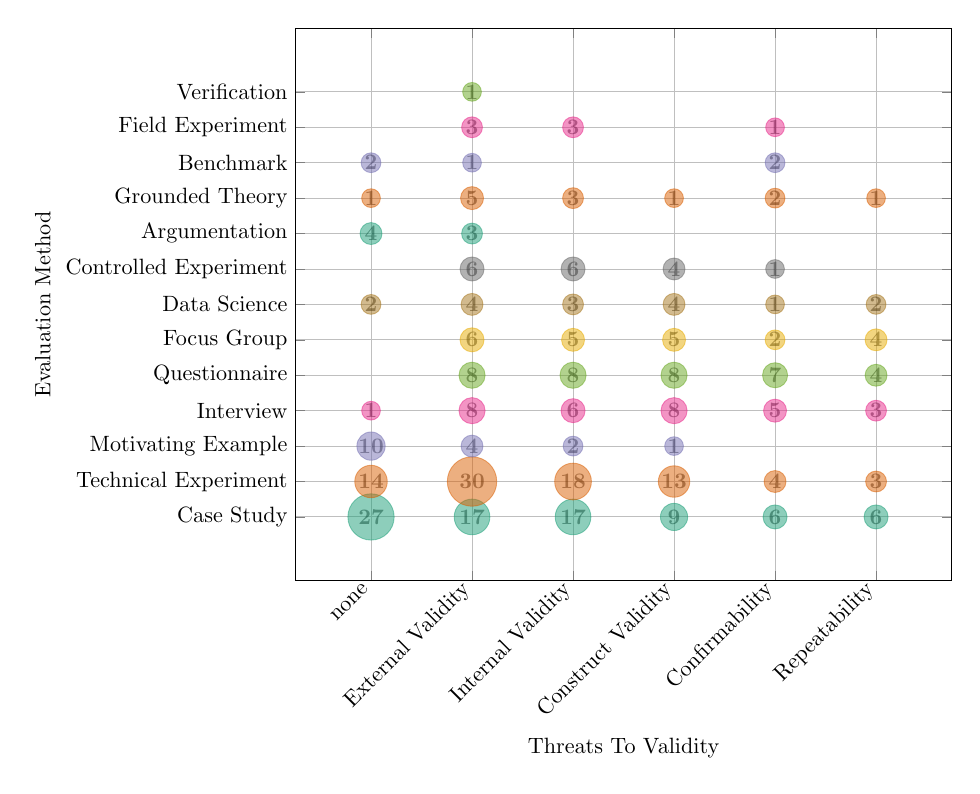
\begin{tikzpicture}[scale=.8]
\pgfplotsset{cycle list/Dark2}
\begin{axis}[width=.99\linewidth,
    enlargelimits=0.15,
    x tick label style={rotate=45,anchor=east},
    xtick={0,1,2,3,4,5}, xticklabels={none,External Validity,Internal Validity,Construct Validity,Confirmability,Repeatability},
    xlabel={Threats To Validity},
    ytick={0,1,2,3,4,5,6,7,8,9,10,11,12}, yticklabels={Case Study,Technical Experiment,Motivating Example,Interview,Questionnaire,Focus Group,Data Science,Controlled Experiment,Argumentation,Grounded Theory,Benchmark,Field Experiment,Verification},
    ylabel={Evaluation Method},
    grid=both,
    scatter,scatter src=y,
    scatter/classes={0={draw=Dark2-A,fill=Dark2-A}, 1={draw=Dark2-B,fill=Dark2-B}, 2={draw=Dark2-C,fill=Dark2-C}, 3={draw=Dark2-D,fill=Dark2-D}, 4={draw=Dark2-E,fill=Dark2-E}, 5={draw=Dark2-F,fill=Dark2-F}, 6={draw=Dark2-G,fill=Dark2-G}, 7={draw=Dark2-H,fill=Dark2-H}, 8={draw=Dark2-A,fill=Dark2-A}, 9={draw=Dark2-B,fill=Dark2-B}, 10={draw=Dark2-C,fill=Dark2-C}, 11={draw=Dark2-D,fill=Dark2-D}, 12={draw=Dark2-E,fill=Dark2-E}}
]

\addplot+[mark=*,mark size=10.448,opacity=0.5,text=black] coordinates { (0,0) } node[text=black,font=\bfseries] {27};
\addplot+[mark=*,mark size=7.343,opacity=0.5,text=black] coordinates { (0,1) } node[text=black,font=\bfseries] {14};
\addplot+[mark=*,mark size=6.388,opacity=0.5,text=black] coordinates { (0,2) } node[text=black,font=\bfseries] {10};
\addplot+[mark=*,mark size=4.239,opacity=0.5,text=black] coordinates { (0,3) } node[text=black,font=\bfseries] {1};
\addplot+[mark=*,mark size=4.478,opacity=0.5,text=black] coordinates { (0,6) } node[text=black,font=\bfseries] {2};
\addplot+[mark=*,mark size=4.955,opacity=0.5,text=black] coordinates { (0,8) } node[text=black,font=\bfseries] {4};
\addplot+[mark=*,mark size=4.239,opacity=0.5,text=black] coordinates { (0,9) } node[text=black,font=\bfseries] {1};
\addplot+[mark=*,mark size=4.478,opacity=0.5,text=black] coordinates { (0,10) } node[text=black,font=\bfseries] {2};
\addplot+[mark=*,mark size=8.060,opacity=0.5,text=black] coordinates { (1,0) } node[text=black,font=\bfseries] {17};
\addplot+[mark=*,mark size=11.164,opacity=0.5,text=black] coordinates { (1,1) } node[text=black,font=\bfseries] {30};
\addplot+[mark=*,mark size=4.955,opacity=0.5,text=black] coordinates { (1,2) } node[text=black,font=\bfseries] {4};
\addplot+[mark=*,mark size=5.910,opacity=0.5,text=black] coordinates { (1,3) } node[text=black,font=\bfseries] {8};
\addplot+[mark=*,mark size=5.910,opacity=0.5,text=black] coordinates { (1,4) } node[text=black,font=\bfseries] {8};
\addplot+[mark=*,mark size=5.433,opacity=0.5,text=black] coordinates { (1,5) } node[text=black,font=\bfseries] {6};
\addplot+[mark=*,mark size=4.955,opacity=0.5,text=black] coordinates { (1,6) } node[text=black,font=\bfseries] {4};
\addplot+[mark=*,mark size=5.433,opacity=0.5,text=black] coordinates { (1,7) } node[text=black,font=\bfseries] {6};
\addplot+[mark=*,mark size=4.716,opacity=0.5,text=black] coordinates { (1,8) } node[text=black,font=\bfseries] {3};
\addplot+[mark=*,mark size=5.194,opacity=0.5,text=black] coordinates { (1,9) } node[text=black,font=\bfseries] {5};
\addplot+[mark=*,mark size=4.239,opacity=0.5,text=black] coordinates { (1,10) } node[text=black,font=\bfseries] {1};
\addplot+[mark=*,mark size=4.716,opacity=0.5,text=black] coordinates { (1,11) } node[text=black,font=\bfseries] {3};
\addplot+[mark=*,mark size=4.239,opacity=0.5,text=black] coordinates { (1,12) } node[text=black,font=\bfseries] {1};
\addplot+[mark=*,mark size=8.060,opacity=0.5,text=black] coordinates { (2,0) } node[text=black,font=\bfseries] {17};
\addplot+[mark=*,mark size=8.299,opacity=0.5,text=black] coordinates { (2,1) } node[text=black,font=\bfseries] {18};
\addplot+[mark=*,mark size=4.478,opacity=0.5,text=black] coordinates { (2,2) } node[text=black,font=\bfseries] {2};
\addplot+[mark=*,mark size=5.433,opacity=0.5,text=black] coordinates { (2,3) } node[text=black,font=\bfseries] {6};
\addplot+[mark=*,mark size=5.910,opacity=0.5,text=black] coordinates { (2,4) } node[text=black,font=\bfseries] {8};
\addplot+[mark=*,mark size=5.194,opacity=0.5,text=black] coordinates { (2,5) } node[text=black,font=\bfseries] {5};
\addplot+[mark=*,mark size=4.716,opacity=0.5,text=black] coordinates { (2,6) } node[text=black,font=\bfseries] {3};
\addplot+[mark=*,mark size=5.433,opacity=0.5,text=black] coordinates { (2,7) } node[text=black,font=\bfseries] {6};
\addplot+[mark=*,mark size=4.716,opacity=0.5,text=black] coordinates { (2,9) } node[text=black,font=\bfseries] {3};
\addplot+[mark=*,mark size=4.716,opacity=0.5,text=black] coordinates { (2,11) } node[text=black,font=\bfseries] {3};
\addplot+[mark=*,mark size=6.149,opacity=0.5,text=black] coordinates { (3,0) } node[text=black,font=\bfseries] {9};
\addplot+[mark=*,mark size=7.104,opacity=0.5,text=black] coordinates { (3,1) } node[text=black,font=\bfseries] {13};
\addplot+[mark=*,mark size=4.239,opacity=0.5,text=black] coordinates { (3,2) } node[text=black,font=\bfseries] {1};
\addplot+[mark=*,mark size=5.910,opacity=0.5,text=black] coordinates { (3,3) } node[text=black,font=\bfseries] {8};
\addplot+[mark=*,mark size=5.910,opacity=0.5,text=black] coordinates { (3,4) } node[text=black,font=\bfseries] {8};
\addplot+[mark=*,mark size=5.194,opacity=0.5,text=black] coordinates { (3,5) } node[text=black,font=\bfseries] {5};
\addplot+[mark=*,mark size=4.955,opacity=0.5,text=black] coordinates { (3,6) } node[text=black,font=\bfseries] {4};
\addplot+[mark=*,mark size=4.955,opacity=0.5,text=black] coordinates { (3,7) } node[text=black,font=\bfseries] {4};
\addplot+[mark=*,mark size=4.239,opacity=0.5,text=black] coordinates { (3,9) } node[text=black,font=\bfseries] {1};
\addplot+[mark=*,mark size=5.433,opacity=0.5,text=black] coordinates { (4,0) } node[text=black,font=\bfseries] {6};
\addplot+[mark=*,mark size=4.955,opacity=0.5,text=black] coordinates { (4,1) } node[text=black,font=\bfseries] {4};
\addplot+[mark=*,mark size=5.194,opacity=0.5,text=black] coordinates { (4,3) } node[text=black,font=\bfseries] {5};
\addplot+[mark=*,mark size=5.672,opacity=0.5,text=black] coordinates { (4,4) } node[text=black,font=\bfseries] {7};
\addplot+[mark=*,mark size=4.478,opacity=0.5,text=black] coordinates { (4,5) } node[text=black,font=\bfseries] {2};
\addplot+[mark=*,mark size=4.239,opacity=0.5,text=black] coordinates { (4,6) } node[text=black,font=\bfseries] {1};
\addplot+[mark=*,mark size=4.239,opacity=0.5,text=black] coordinates { (4,7) } node[text=black,font=\bfseries] {1};
\addplot+[mark=*,mark size=4.478,opacity=0.5,text=black] coordinates { (4,9) } node[text=black,font=\bfseries] {2};
\addplot+[mark=*,mark size=4.478,opacity=0.5,text=black] coordinates { (4,10) } node[text=black,font=\bfseries] {2};
\addplot+[mark=*,mark size=4.239,opacity=0.5,text=black] coordinates { (4,11) } node[text=black,font=\bfseries] {1};
\addplot+[mark=*,mark size=5.433,opacity=0.5,text=black] coordinates { (5,0) } node[text=black,font=\bfseries] {6};
\addplot+[mark=*,mark size=4.716,opacity=0.5,text=black] coordinates { (5,1) } node[text=black,font=\bfseries] {3};
\addplot+[mark=*,mark size=4.716,opacity=0.5,text=black] coordinates { (5,3) } node[text=black,font=\bfseries] {3};
\addplot+[mark=*,mark size=4.955,opacity=0.5,text=black] coordinates { (5,4) } node[text=black,font=\bfseries] {4};
\addplot+[mark=*,mark size=4.955,opacity=0.5,text=black] coordinates { (5,5) } node[text=black,font=\bfseries] {4};
\addplot+[mark=*,mark size=4.478,opacity=0.5,text=black] coordinates { (5,6) } node[text=black,font=\bfseries] {2};
\addplot+[mark=*,mark size=4.239,opacity=0.5,text=black] coordinates { (5,9) } node[text=black,font=\bfseries] {1};


\end{axis}
\end{tikzpicture}
\end{center}
%\caption{Portfolio f\"ur Threats To Validity und Evaluation Method (Gr\"o\ss{}e entspricht der Anzahl)}\label{fig:port_threatstovalidity_evaluationmethod}
%\end{figure}



\section{Relations between evaluation methods (per research object) and kind of provided artifact (per paper)}

\input{figs/port_artifacts_evaluationmethod}

%\bibliographystyle{unsrt}
%\bibliography{ECSA-ICSA-Proceedings}

\end{document}

